\documentclass[ukrainian,14pt]{extarticle}
% \documentclass[english,14pt]{extarticle}
%\documentclass[14pt]{
\usepackage{chngcntr}
% \usepackage[british]{babel}

\counterwithin*{equation}{section}
% \counterwithin*{equation}{subsection}

\usepackage{svg}
\usepackage{babel}
\usepackage[utf8]{inputenc}
\usepackage{fullpage}
\usepackage{breqn}
\usepackage{ upgreek }
\usepackage{amsmath}
\usepackage{pifont}
\usepackage[bookmarks=true]{hyperref}
\usepackage{bookmark}
\usepackage{graphicx}
\usepackage{tocloft}
\usepackage{listings}
\usepackage{indentfirst}

\usepackage{listings}
\usepackage{color}
\usepackage{titlesec}
\titlelabel{\thetitle.\quad}
 
\definecolor{codegreen}{rgb}{0,0.6,0}
\definecolor{codegray}{rgb}{0.5,0.5,0.5}
\definecolor{codepurple}{rgb}{0.58,0,0.82}
\definecolor{backcolour}{rgb}{0.95,0.95,0.92}

\counterwithin{equation}{section}

\lstdefinestyle{mystyle}{
    backgroundcolor=\color{backcolour},   
    commentstyle=\color{codegreen},
    keywordstyle=\color{magenta},
    numberstyle=\tiny\color{codegray},
    stringstyle=\color{codepurple},
    basicstyle=\footnotesize,
    breakatwhitespace=false,         
    breaklines=true,                 
    captionpos=b,                    
    keepspaces=true,                 
    numbers=left,                    
    numbersep=5pt,                  
    showspaces=false,                
    showstringspaces=false,
    showtabs=false,                  
    tabsize=2
}
 
\lstset{style=mystyle}




\renewcommand\cftsecleader{\cftdotfill{\cftdotsep}}


\def\ab{[a,b]}
\newcommand{\sign}{\operatorname{sign}}

\begin{document}




% \setcounter{section}{2}
% \setcounter{page}{24}
% \section{Опис програми і отриманих результатів}
% \subsection{Призначення програми}

% Програма призначена для побудови апроксимацій функцій чебишовськими сплайнами. Функція може бути задана двома способами: дискретним (у вигляді таблиці) або аналітично. Програма дає змогу знайти коефіцієнти многочленів чебишовського наближення, границі кожної ланки сплайна, максимальні похибки на кожній ланці сплайну. А також будувати графіки сплайна, яким наближуємо функцію, функції, яка наближується, графік функції похибки. Є можливість порівняти два наближення для певної функції. 

% \subsection{Умови застосування}
% Вимоги до ПК:

% \begin{itemize}
%   \item 32-розрядний (x86) або 64-розрядний (x64) процесор із тактовою частотою 1 ГГц або швидший;
%   \item 1 гігабайт (ГБ) RAM (для 32-розрядної версії) або 2 ГБ (для 64-розрядної версії);Another entry in the list
% \end{itemize}
% ОС: Windows 7/8/10

% \subsection{Запуск програми та задання вхідних даних}
% Для знаходження наближення функції, спочатку потрібно вибрати, яким чином задана функція (таблично чи аналітично). Це можна зробити натиснувши кнопку з правої сторони головного меню сайту.

% \vspace{0.5cm}
% 
\includegraphics[scale=1]{program_screenshots/hamburger.png}


% Далі необхідно вибрати метод яким потрібно апроксимувати функцію.
% \vspace{0.5cm}

% 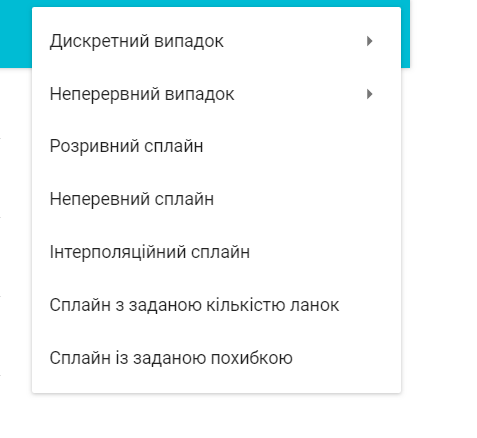
\includegraphics[scale=1]{program_screenshots/approximation_options.png}


% Для неперервного випадку, потрібно заповнити наступну форму:

% 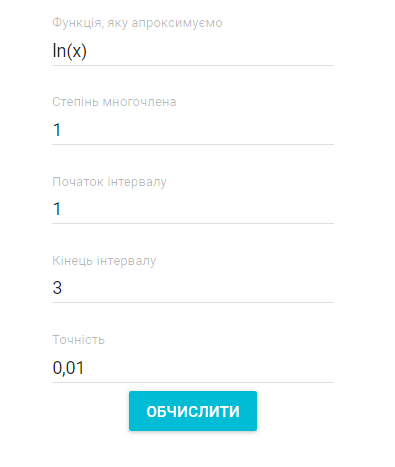
\includegraphics[scale=1]{program_screenshots/form.png}


% Як видно з рисунку, користувачу потрібно вибрати функцію для апроксимації. Приклади вводу функцій:

% \bgroup
% \def\arraystretch{1.5}%  1 is the default, change whatever you need
% \begin{center}
% \begin{tabular}{ c | c }
%  $e^x$ & e^x \\
%  \hline
%  $\sqrt(x)$ & sqrt(x) \\
%  \hline
%  $cos^2(x)$ & cos(x)^2 або (cos(x))^2 \\
%  \hline
%  $\frac{1}{x}$ & 1/x
% \end{tabular}
% \end{center}
% \egroup

% Точність – допустима відносна похибка у визначенні похибки наближення у мінімаксному наближенні.
% Для дискретного випадку:

% 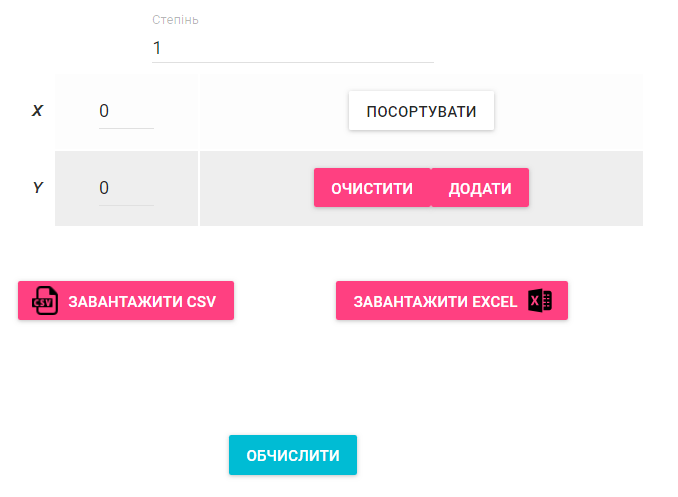
\includegraphics[scale=1]{program_screenshots/form_discrete.png}

% Тут можна задати степінь апроксимуючого многочлена та задати табличну функцію. Це можна зробити двома способами:
% \begin{enumerate}
%     \item Вручну. За допомогою кнопки “ДОДАТИ ТОЧКУ” можна додати до таблиці, яка знаходиться лівіше, ще одну точку. Редагувати точки можна відразу в таблиці. При необхідності можна також вилучити точку навівши курсор на неї.

% 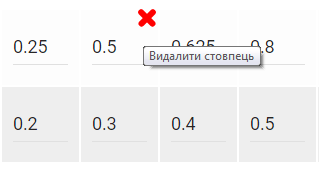
\includegraphics[scale=1]{program_screenshots/delete_point.png}

% Також є можливість посортувати ці точки (по змінній x), натиснувши на відповідну кнопку.

%     \item  Завантажити з файлу. Файл повинен бути у форматі CSV(Comma Separated Values), тобто значення які розділені комою. Перший стовпець – це значення x, другий – y. Приклад файлу CSV: 
% \vspace{0.5cm}

% 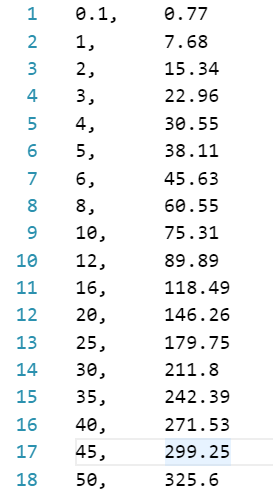
\includegraphics[scale=1]{program_screenshots/points.png}

% Також файл може бути у форматі xlsx (Excel). Приклад Excel файлу.

% 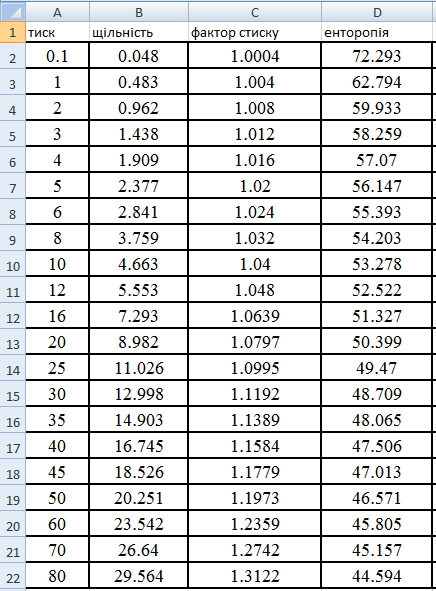
\includegraphics[scale=1]{program_screenshots/excel.png}
% \end{enumerate}

% Далі необхідно вибрати яка величина – змінна x, а яка – y.

% 
\includegraphics[scale=1]{program_screenshots/x_y_chooser.png}

% Після цього, незважаючи на спосіб, яким задали функцію (вручну чи завантажили з файлу), потрібно натиснути кнопку “ОБЧИСЛИТИ”. Коли запит обробиться на сервері, результати можна побачити на екрані.

% \subsection{Опис отриманих результатів}

% Приклад отриманих результатів наближення функції $sin(x)$, розривним лінійним сплайном на проміжку $[1, 5]$ із заданою похибкою на кожній ланці – $0.1$. Вхідні дані:

% 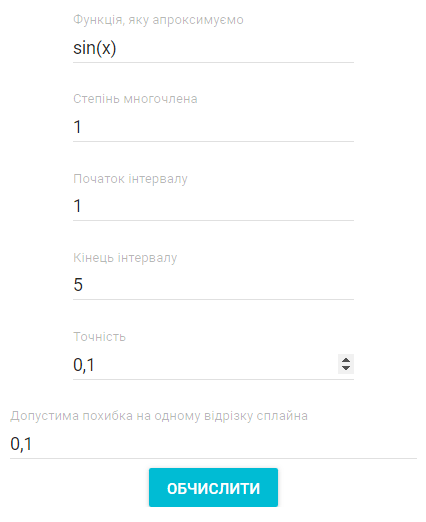
\includegraphics[scale=1]{program_screenshots/form_example.png}

% Вихідні дані:

% 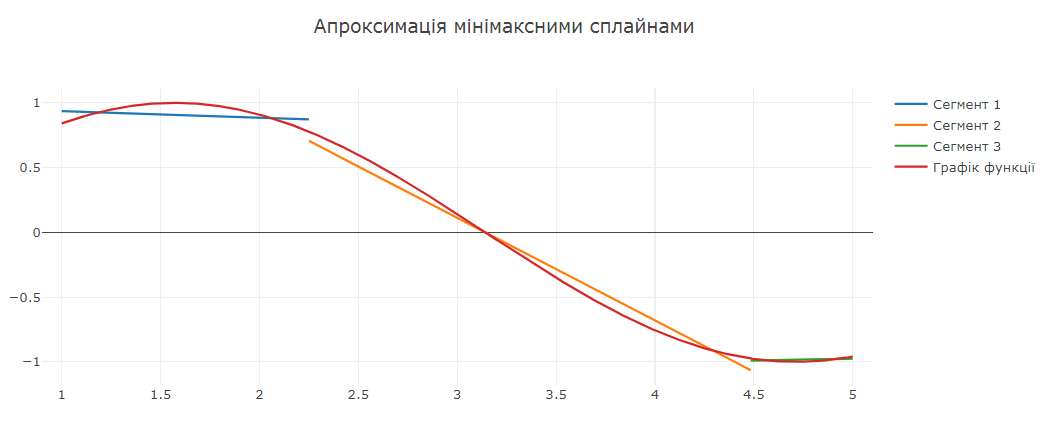
\includegraphics[scale=0.6]{program_screenshots/approx_example_3_4.png}

% Як можна побачити з рисунку, результатом роботи програми є вивід на екран графік функції, яку наближаємо, а також сплайна. 

% 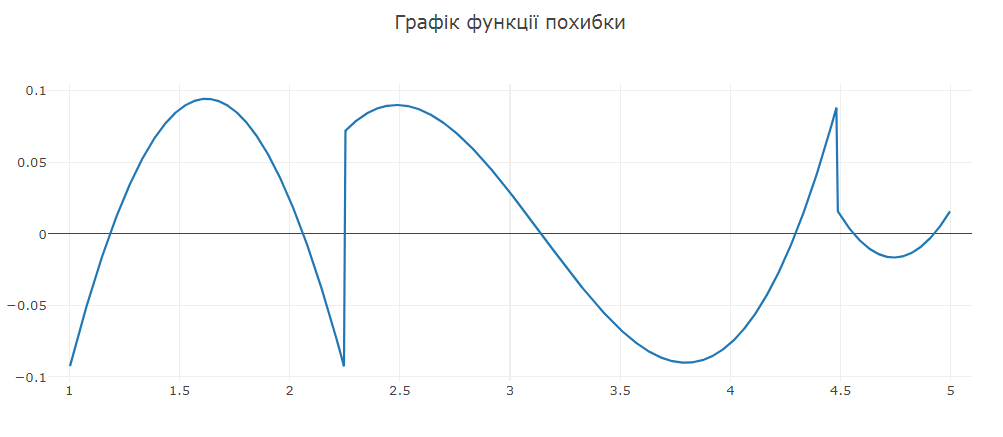
\includegraphics[scale=0.6]{program_screenshots/error_example_3_4.png}

% Також виводиться графік функції похибки на кожній ланці.

% 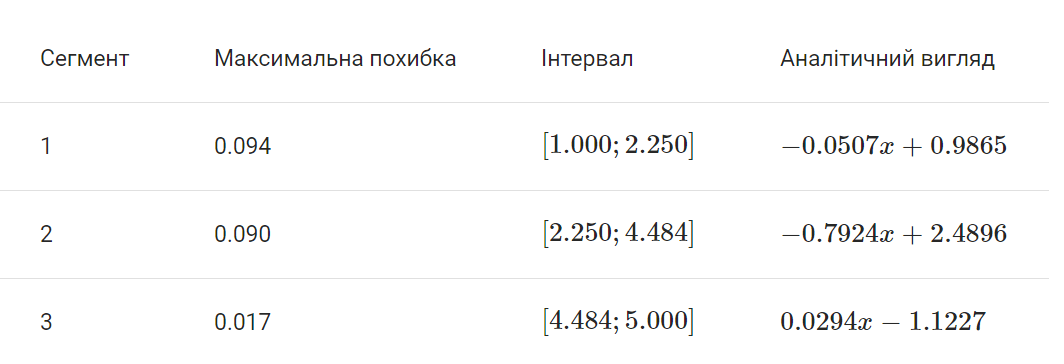
\includegraphics[scale=0.5]{program_screenshots/example_table_result.png}

% В таблиці представлено максимальну похибку, межі інтервалу і аналітичний вигляд многочлена на всіх ланках чебишовського сплайна. 


% \newpage
% \setcounter{page}{37}

% \section*{Додатки}
% \addcontentsline{toc}{section}{Додатки}

% \subsection*{Додаток 1. Код програми}
% \addcontentsline{toc}{subsection}{Додаток 1. Код програми}

% Підпрограма для створення початкового альтернанcу (дискретний випадок).
% Вхідні параметри:
% \begin{enumerate}
%     \item масив значень x
%     \item degree – степінь апроксимуючого многочлена
% \end{enumerate}
% Результат виконання функції: початковий альтернанс
% В цій функції використана бібліотека numpy(http://www.numpy.org/).


% \lstinputlisting[language=Python]{code/make_initial_alternance.py}

% \vspace{1cm}

% Підпрограма для визначення максимального значення функції в дискретних точках.
% Вхідні параметри:
% \begin{enumerate}
%     \item func – функція
%     \item  x_vals – масив дискретних точок
% \end{enumerate}
% Результат виконання функції: максимальне значення заданої функції

% \lstinputlisting[language=Python]{code/max_error.py}
% \vspace{1cm}


% Підпрограма для заміни точок альтернансу.
% Вхідні параметри:
% \begin{enumerate}
%     \item err_func – функція похибки
%     \item alternance – попередній альтернанс
%     \item  x_vals – значення x для таблично заданої функції
% \end{enumerate}
% Результат виконання функції: новий альтернанс
% \lstinputlisting[language=Python]{code/change_alternance.py}
% \vspace{1cm}

% Підпрограма для побудови аналітичного вигляду многочлена.
% Вхідні параметри:
% \begin{enumerate}
%     \item t – альтернанс
%     \item degree – степінь апроксимуючого многочлена
%     \item f_discrete – дискретна функція
% \end{enumerate}
% Результат виконання функції: аналітичний вигляд многочлена.

% \lstinputlisting[language=Python]{code/pol.py}

% \vspace{1cm}

% Підпрограма \textit{main} для апроксимації чебишовським сплайном з заданою кількістю ланок.
% Вхідні параметри:
% \begin{enumerate}
%     \item func – функція, яку апроксимуємо
%     \item deg – степінь апроксимуючого многочлена
%     \item start – початок інтервалу
%     \item end – кінець інтервалу
%     \item r – кількістю ланок
% \end{enumerate}

% \lstinputlisting[language=Python]{code/with_specified_number_of_segments.py}
% \newpage

\setcounter{page}{41}
\subsection*{Додаток 2. Результати виконання програми}
\addcontentsline{toc}{subsection}{Додаток 2. Результати виконання програми }

\textbf{Приклад 1.} Знайти рівномірне наближення чебишовським інтерполяційним сплайном третього степеня для функції $f(x) = 4sin(x) \sqrt{x}$ на проміжку $[0, 2\pi]$ із заданою похибкою – $0.03$.


Результат роботи програми:
\vspace{0.5cm} \\

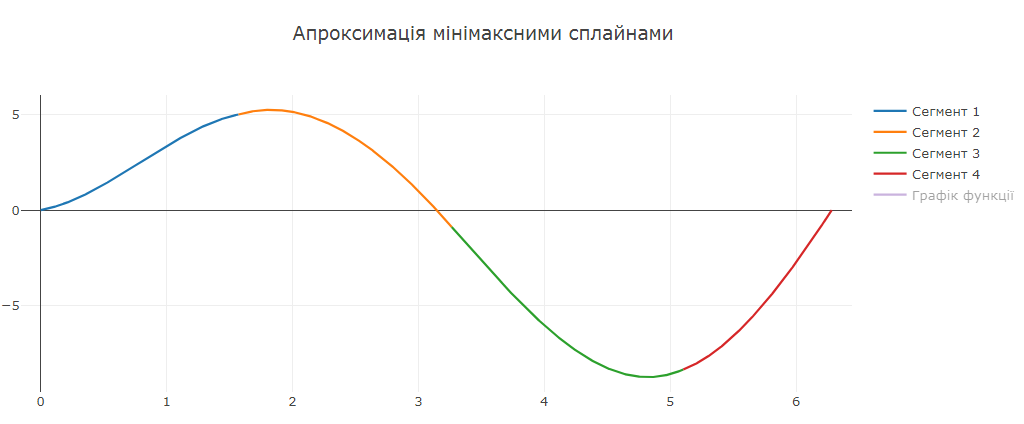
\includegraphics[scale=0.65]{examples/1_approx.png}
\vspace{0.5cm}
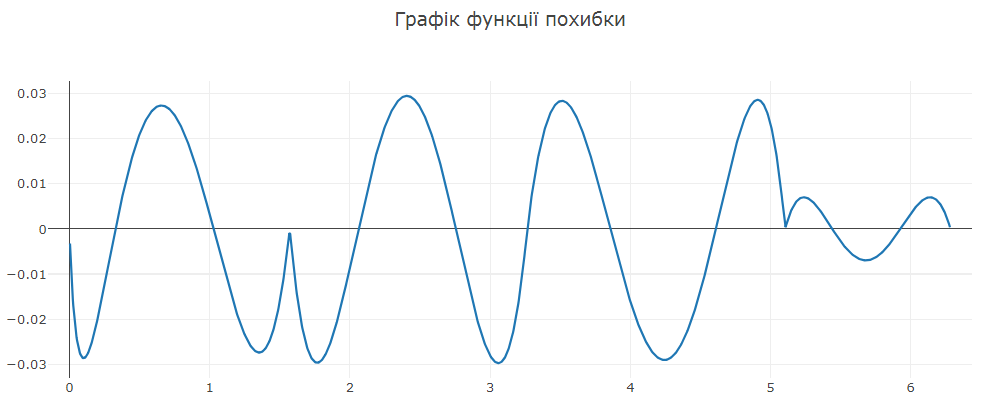
\includegraphics[scale=0.65]{examples/1_error.png}
\vspace{0.5cm}
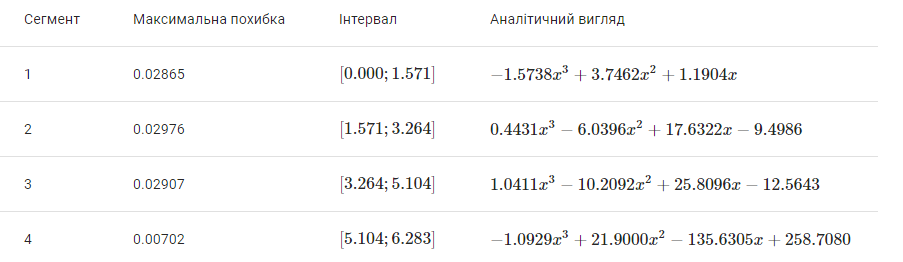
\includegraphics[scale=0.7]{examples/1_table.png}

\vspace{1cm}
\textbf{Приклад 2.} Знайти рівномірне наближення розривним чебишовським сплайном третього степеня для функції $f(x)=4*sin(x) \sqrt{x} $ на проміжку $[0, 2\pi]$ із заданою похибкою – $0.03$.

Результат роботи програми:
\vspace{0.5cm} \\
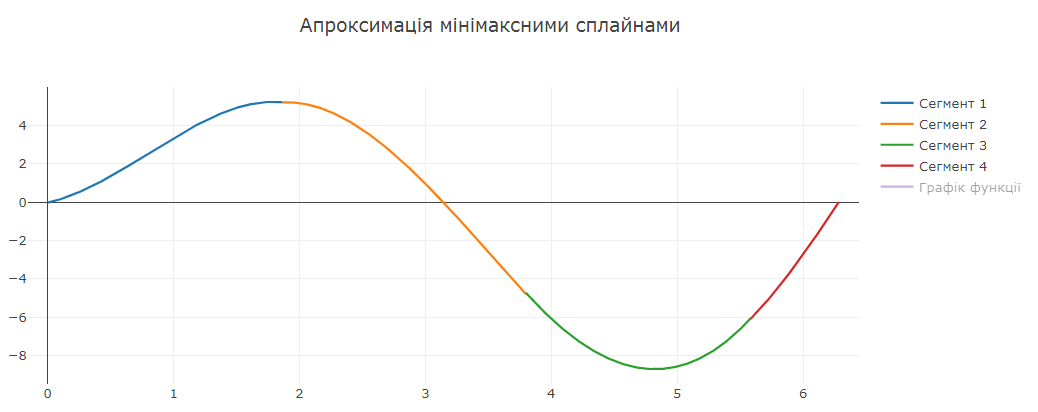
\includegraphics[scale=0.65]{examples/2_approx.png}
\vspace{0.5cm}
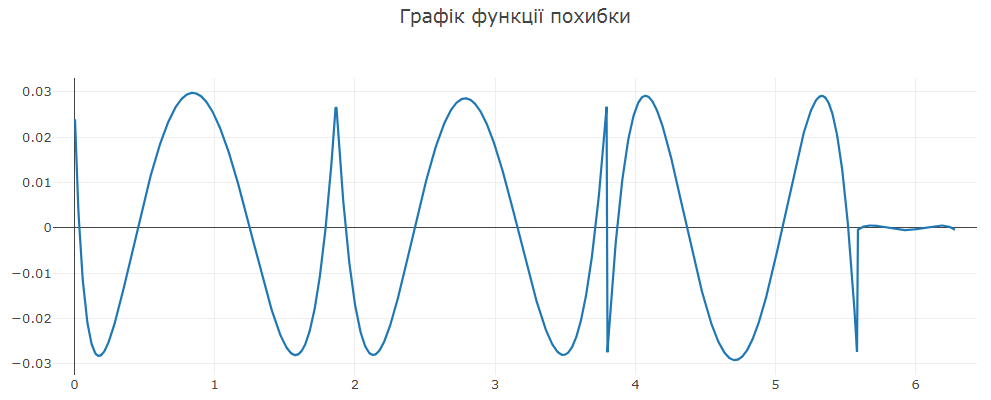
\includegraphics[scale=0.65]{examples/2_error.png}
\vspace{0.5cm}
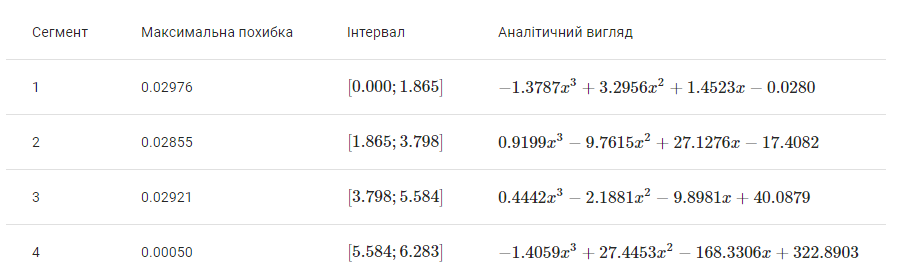
\includegraphics[scale=0.7]{examples/2_table.png}
\vspace{1cm}

\newpage
\textbf{Приклад 3.} Знайти рівномірне наближення чебишовським інтерполяційним сплайном 2-го степеня функції $f(x)=e^x$ на проміжку $[0, 3]$ з заданою кількістю ланок - $3$.

Результат роботи програми:
\vspace{0.5cm} \\
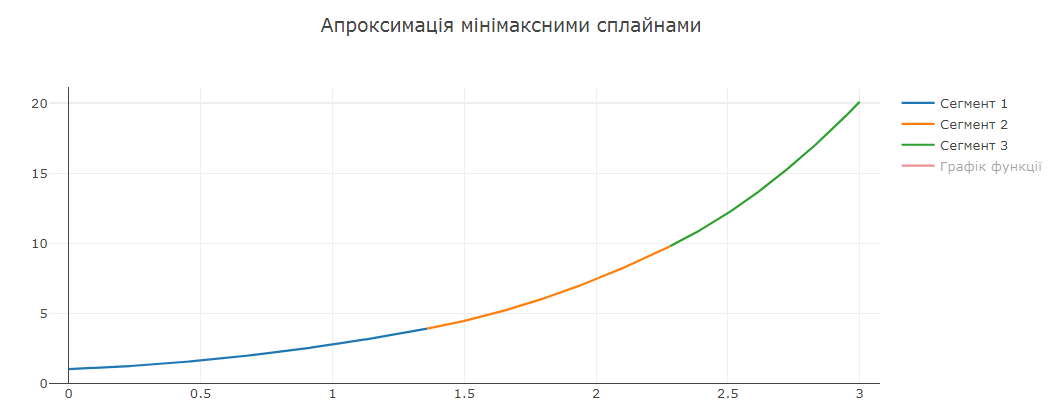
\includegraphics[scale=0.65]{examples/3_approx.png}

\vspace{0.5cm}

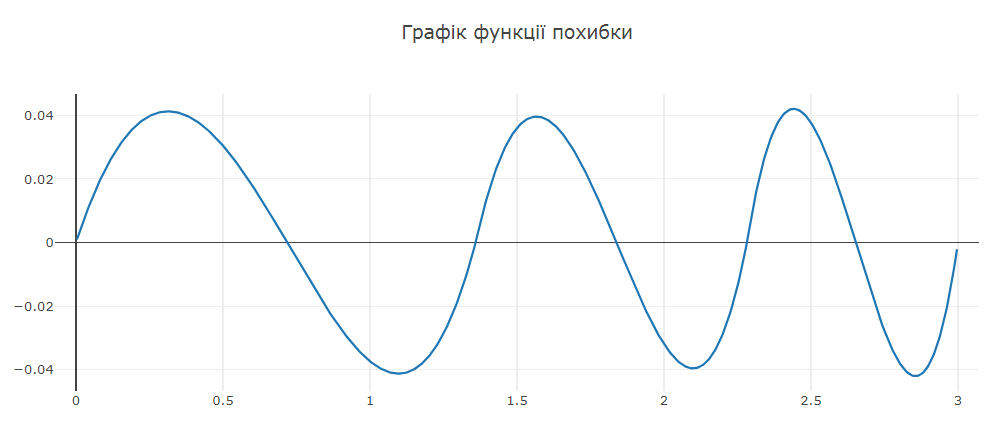
\includegraphics[scale=0.65]{examples/3_error.png}

\vspace{0.5cm}

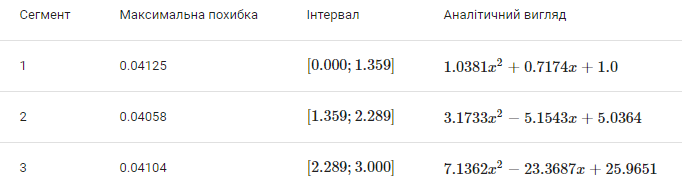
\includegraphics[scale=0.8]{examples/3_table.png}

\vspace{1cm}

\newpage
\textbf{Приклад 4.} Знайти рівномірне наближення чебишовським розривним сплайном 2-го степеня функції $f(x)=e^x$ на проміжку $[0, 3]$ з заданою кількістю ланок - $3$.
Результат роботи програми:
\vspace{0.5cm} \\
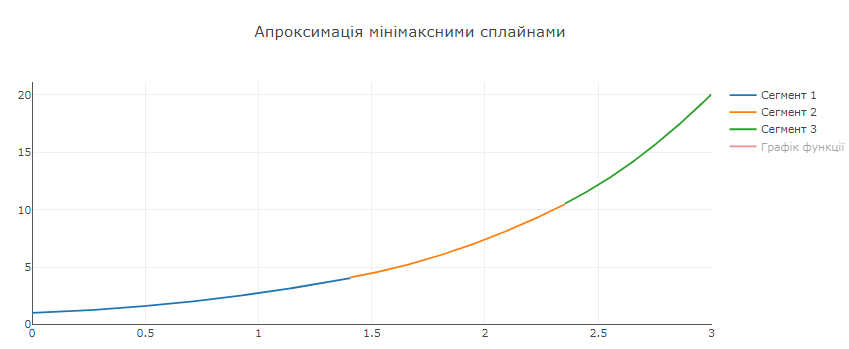
\includegraphics[scale=0.65]{examples/4_approx.png}
\vspace{0.5cm}
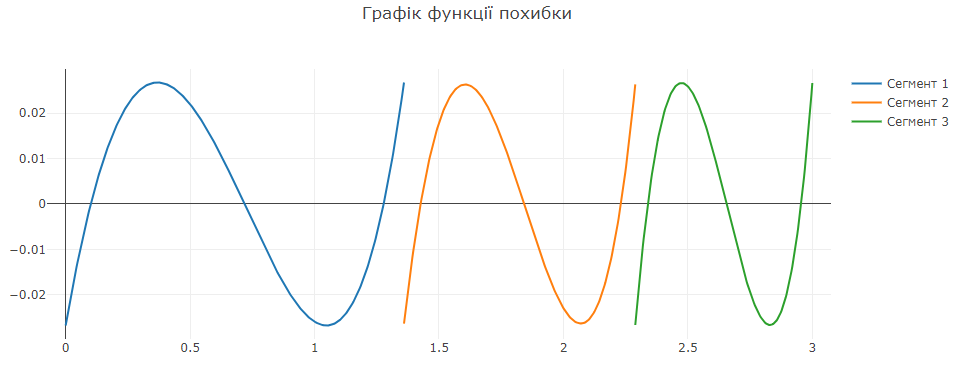
\includegraphics[scale=0.7]{examples/4_error.png}
\vspace{0.5cm}
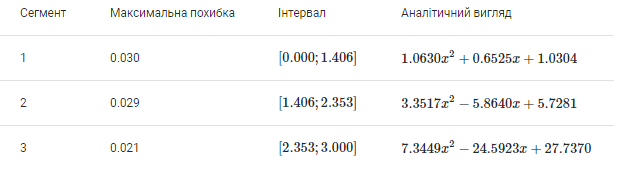
\includegraphics[scale=0.65]{examples/4_table.png}


\end{document}